\documentclass{article}

%opening
\title{Manco il titolo mi ricordo}
\author{Cristina Caprioglio}
\date{2023/2024 }
\usepackage[margin=0.75in]{geometry}
	\usepackage{amssymb}
	\usepackage{amsmath}
	\usepackage{multicol}
	\usepackage{graphicx}
	\usepackage{physics}
	\usepackage{subcaption}
	\usepackage{float}
	\usepackage[justification=centering]{caption}
\begin{document}

\maketitle

\section*{Introduction}
Scopo+descrizione sistema
\section{Hydrostatic configuration}
\subsection{Physical model}
The first part of the project is about understanding how the gas is distributed in a cluster, so to do a proper gravitational model is needed.
We'll assume spherical symmetry, which will lead to all physical quantities depending only on $r$, the radial coordinate, which indicates the distance from the centre of the system.
The gas is supported by thermal pressure and it's described by the hydrostatic equilibrium equation:
\begin{equation}\label{idro_eq}
	\derivative{P}{r}=-\frac{GM(<r)}{r^{2}}\rho_{g}(r),
\end{equation}
which is a I order ODE. We have that in \eqref{idro_eq} $M(<r)$ indicates the total mass contained in a radius $r$, not just the mass of the gas, while $P$ and $\rho_{g}$ refer to the pressure and the density of the gas. \\
We have that the ICM is in equilibrium in the gravitational potential of the cluster, which is dominated by dark matter. \\
For the density profile of the latter we will assume a $Navarro-Frenk-White$ (NFW) $profile$, which takes the following form:
\begin{equation}\label{NFW}
	\rho_{DM}(r)=\frac{\rho_{DM,0}}{\left(\frac{r}{r_{s}}\right)\left(1+\frac{r}{r_{s}}\right)^{2}},
\end{equation}
where $\rho_{DM,0}$ and $r_{s}$ are parameters which depend on the cluster mass. 
Integrating \eqref{NFW} we can calculate the mass profile, which as an analytical solution:
\begin{equation}\label{massDM}
	M_{DM}(r)=\int_{0}^{r}4\pi r'^{2}\rho_{DM}(r')\dd{r'}=4\pi\rho_{DM,0}r_{s}^{3}\left[\ln\left(1+\frac{r}{r_{s}}\right)-\frac{r/r_{s}}{1+r/r_{s}}\right].
\end{equation}
To have a more realistic model we will also need to consider the presence of the BCG. Its stellar mass is described by the $Hernquist\; profile$:
\begin{equation}\label{Hern}
	M_{*}(r)=M_{BCG}\frac{r^{2}}{(r+a)^{2}},
\end{equation}
where $M_{BCG}$ is the mass of the elliptical central galaxy and $a$ is a scale related to the half-mass radius $r_{1/2}$: $r_{1/2}=(1+\sqrt{2})a$.\\
Assuming the ICM is described by the perfect gas equation of state (i.e. $P=\frac{k_{B}\rho_{g}T_{g}}{\mu m_{p}}$), \eqref{idro_eq} becomes:
\begin{equation}\label{hydroperf}
	\derivative{\ln \rho_{g}}{r}=-\frac{GM(<r)}{r^{2}}\frac{\mu m_{p}}{k_{B}T_{g}(r)}-\derivative{\ln T_{g}}{r},
\end{equation}
where $T_{g}(r)$ is the gas temperature, while $\mu ,\, m_{p},$ and $k_{B}$ are constants that represent the mean molecular weight, the proton mass and the Boltzmann constant respectively.\\
In the case of an isothermal gas and in the absence of the BCG eq.\eqref{hydroperf} has an analytical solution:
%\begin{equation}
	\begin{gather}\label{isogas}
		\rho_{g}=\rho_{0}\exp\left\{-\frac{27}{2}b\left[1-\frac{\ln (1+r/r_{s})}{r/r_{s}}\right]\right\}=\rho_{0}e^{-27b/2}\left(1+\frac{r}{r_{s}}\right)^{27b/(2r/r_{s})},\\
	with \quad b=\frac{8\pi G\mu m_{p}\rho_{DM,0}r_{s}^{2}}{27k_{B}T_{g,iso}}\notag
	\end{gather}
%\end{equation}
\subsection{The simulation}
The first step is building two uniform grids, with one shifted by $\frac{1}{2}\Delta r$, where $\Delta r=r\textsubscript{j}-r\textsubscript{j-1}$. The maximum number of points in the grids is $j\textsubscript{max}=5000$, while $r$ ranges from $r\textsubscript{min}=0 Mpc$ to $r\textsubscript{max}=3 Mpc$.
The points for the first grid are going to be
\begin{equation}
	r_{j}=r_{min}+\frac{j-1}{j_{max}-1}r_{max},\qquad 1\le j\le j_{max}
\end{equation}
so we'll use integer numbers to refer to them, while we'll use half-integers for the points in the second one.
We'll thus need to define not only the points but also $r_{jmax+1/2}$, which we'll do as follows:
\begin{equation}
	\begin{cases}
		r_{jmax+1/2}=r\textsubscript{jmax-1/2}+(r\textsubscript{jmax-1/2}-r\textsubscript{jmax-3/2})\\
		r\textsubscript{j+1/2}=r\textsubscript{j}+\frac{r\textsubscript{j+1}-r\textsubscript{j}}{2} \qquad 1\le j\le j_{max}-1
	\end{cases}
\end{equation}
Both the temperature $T$ and the density $\rho$ are centered at $r\textsubscript{j+1/2}$, while we centered the mass to $r\textsubscript{j}$.\\
To proceed with the simulation, we first integrate numerically $\rho\textsubscript{DM}$ in order to get $M\textsubscript{DM}$.
Assuming $ M\textsubscript{DM,1}=0$, we get the following expression:
\begin{equation}
	M\textsubscript{DM,j}=M\textsubscript{DM,j-1}+\rho\textsubscript{DM,j-1/2}\Delta V\textsubscript{j},
\end{equation}
where the j-th volume element $\Delta V\textsubscript{j}$ is given by:
\begin{equation}
	\Delta V\textsubscript{j}=\frac{4}{3}\pi(r^{3}_{j}-r^{3}_{j-1}).
\end{equation}
To check the integration we overplotted the results against the analytical solution found in \eqref{massDM}.\\
Once obtained $M_{DM}$ we can move on to the integration of \eqref{hydroperf}. We consider three possible scenarios:
\begin{itemize}
	\item isothermal gas without the presence of the BCG, where we have $\derivative{\ln T_{g}}{r}=0$ and $M_{j}=M_{DM,j}$;
	\item isothermal gas with the presence of the BCG, where we have $\derivative{\ln T_{g}}{r}=0$ and $M_{j}=M_{DM,j}+M_{*,j}$;
	\item non-isothermal gas with the presence of the BCG, where we have $\derivative{\ln T_{g}}{r}\ne 0$ and $M_{j}=M_{DM,j}+M_{*,j}$;
\end{itemize}
We transform \eqref{hydroperf} from an ODE to a FDE (finite difference equation), with the derivative centered in $j$:
\begin{equation}\label{11}
	\frac{\ln \rho_{g,j+1/2}-\ln \rho_{g,j-1/2}}{r_{j+1/2}-r_{j-1/2}}=-\frac{\mu m_{p}}{k_{B}\overline{T}_{g,j}}\frac{GM_{j}}{r_{j}^{2}}-\frac{\ln T_{g,j+1/2}-\ln T_{g,j-1/2}}{r_{j+1/2}-r_{j-1/2}},
\end{equation}
where $\overline{T}_{g,j}$ is defined as $\frac{T_{g,j+1/2}-T_{g,j-1/2}}{2}$. The expression for $\ln \rho_{g,j+1/2}$ can then be easily found from \eqref{11}:
\begin{equation} \label{numrho}
	\ln\rho_{g,j+1/2}=\ln\rho_{g,j-1/2}-\Delta r\frac{\mu m_{p}}{k_{B}\overline{T}_{g,j}}\frac{GM_{j}}{r_{j}^{2}}-(\ln T_{g,j+1/2}-\ln T_{g,j-1/2}).
\end{equation}
To find the appropriate values for the initial condition of the gas density we first run the code with an initial guess with the expected order of magnitude, then we adjust rthe values in order
to obtain a baryon fraction $f_{b}=\frac{M_{*}+M_{gas}}{M_{*}+M_{gas}+M_{DM}}$ close to the cosmic value ($\sim 0.16$) at the virial radius of the cluster ($r_{vir}\approx 2.8$ Mpc).\\
To conclude the setting of the simulations, the following list contains the parameters value and the temperature profiles:
\begin{itemize}
	\item for the NFW profile: $\rho_{DM,0}=7.35\times 10^{-26}$ g/cm$^{3}$ and $r_{s}=435.7$ kpc;
	\item for the $Hernquist$ $ profile$: $M_{BCG}=10^{12} M_{\odot}$ and $r_{1/2}=12$kpc;
	\item the initial condition $\rho_{g,0}$ for the gas density and the respective $f_{b}$ are: \begin{itemize}
		\item $4.1\times 10^{-26}$g/cm$^{3}$ and $0.159$ for the first scenario;
		\item $8\times 10^{-26}$g/cm$^{3}$ and $0.159$ for the second;
		\item $1.5\times 10^{-25}$g/cm$^{3}$ and $0.160$ for the third;
	\end{itemize}
	\item for both temperature pofiles we have $\mu=0.61$, while their expressions are:
	\begin{itemize}
		\item for the isothermal case: $T_{g}=T_{mg}=8.9\times 10^{7}$K;
		\item for the non-isothermal one:
		\begin{equation}\label{Tprof}
			\frac{T_{g}}{T_{mg}}=1.35\frac{(x/0.045)^{1.9}+0.45}{(x/0.045)^{1.9}+1}\frac{1}{(1+(x/0.6)^{2})^{0.45}}
		\end{equation}
		where $x=r/r_{500}$, with $r_{500}\sim r_{vir}/2=1.4$Mpc.
	\end{itemize}
\end{itemize}


\subsection{Results and discussion}
First we compare the analytical NFW mass profile to the numerical one, as well as to the Hernquist mass profile. These are plotted in Fig.\ref{fig:massprofiles}, and we can see how the analytical and numerical mass profile for dark matter barely differ, with a separation only noticeable in the first $2$ kpc.
\begin{figure}[H]
	
	\begin{subfigure}{0.49\textwidth}
		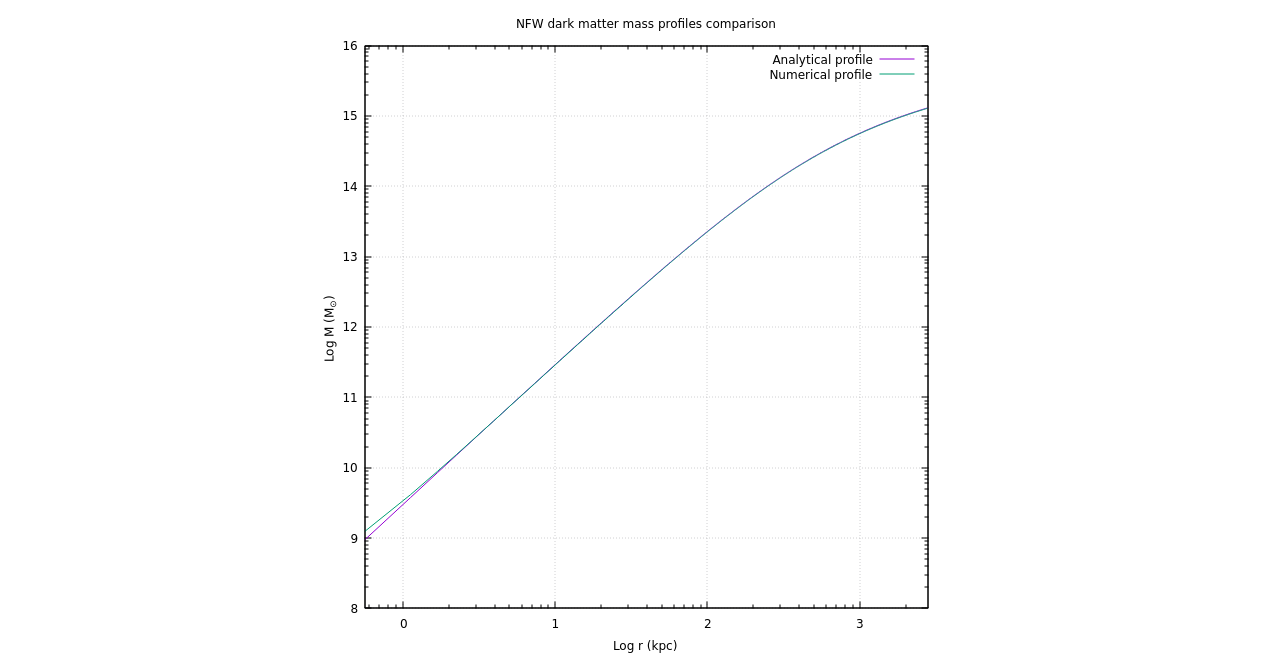
\includegraphics[width=0.9\linewidth]{dm_mass_profile.png}
	\end{subfigure}
	\begin{subfigure}{0.49\textwidth}
		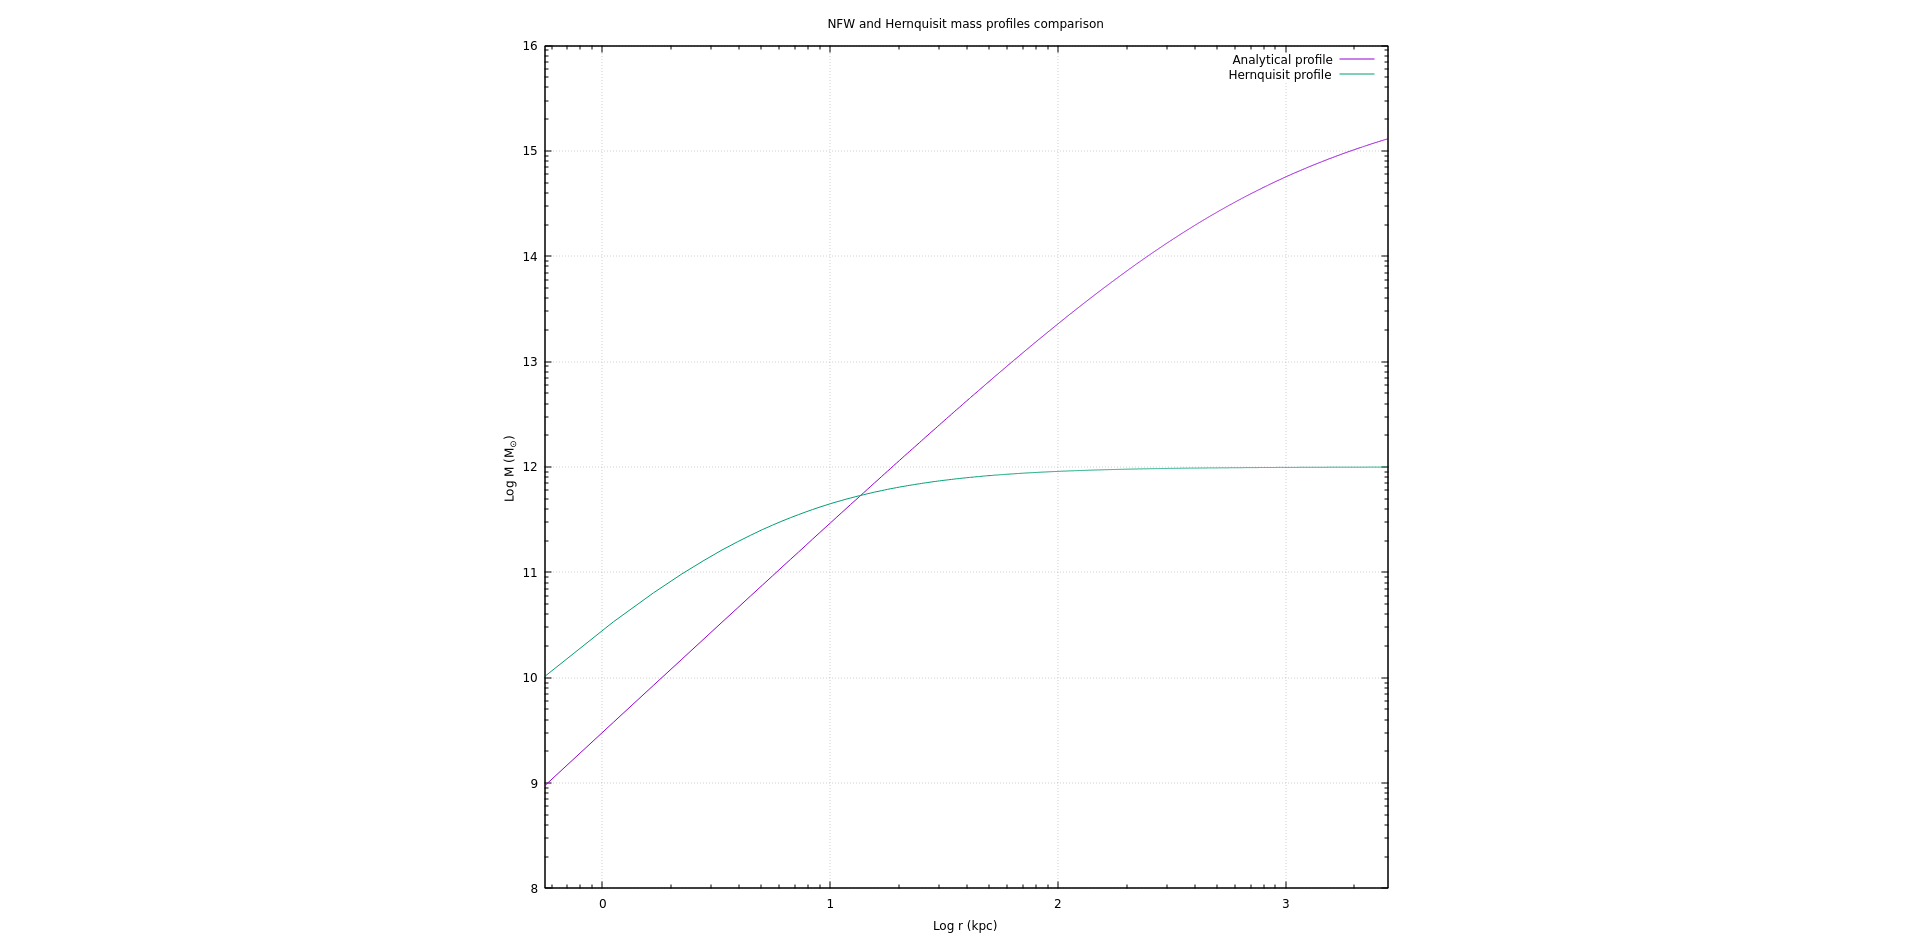
\includegraphics[width=0.9\linewidth]{mass_profiles.png}
	\end{subfigure}
	\centering
	\caption{On the left: analytical (purple curve) and numerical (green curve) NFW profiles. \\On the right: analitycal NFW (purple curve) and Hernquist (green curve) mass profiles.}
	\label{fig:massprofiles}
\end{figure}
In Fig.\ref{fig:densityprofiles} we plot the different density profiles, obtained through the numerical integration of \eqref{hydroperf} through \eqref{numrho}. \\
Comparing the isothermal models, we can notice how the presence of the BCG causes a steepening of the density profile in the
central regions. This is because of the term $\frac{GM(r)}{r^{2}}$ present in \eqref{hydroperf}, which represents the gravitational field, which increases with the presence of the BCG.
This is also the reason why you need to increase $\rho_{0}$ in order to keep the baryon fraction at $0.16$.\\
As for the differences between the isothermal model and the one with the temperature gradient, before we comment on the differences it's better to show the different temperature profiles, which is done in Fig.\ref{fig:tempprof}.
\begin{figure}[H]
	\centering
	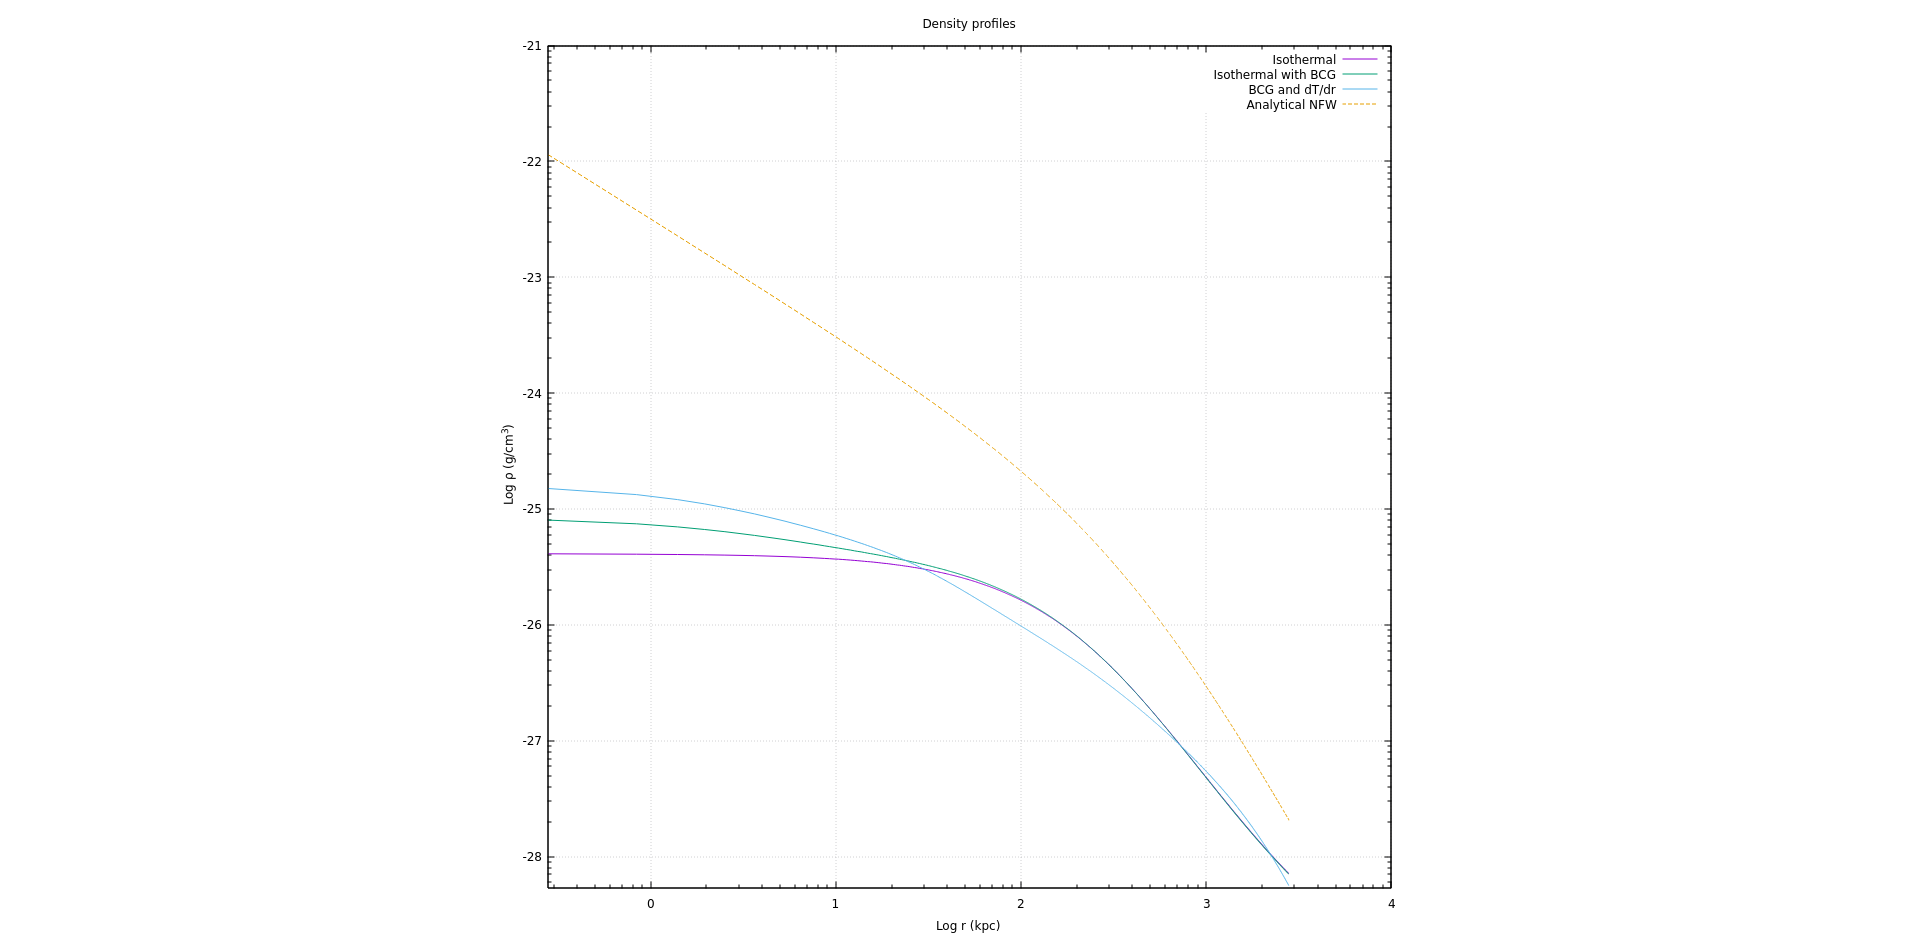
\includegraphics[width=\textwidth]{density_profiles.png}
	\caption{The different density profiles obtained from \eqref{hydroperf} for the following models: with only dark matter and isothermal gas (purple curve), with also the BCG but still isothermal (green curve), and with BCG and temperature gradient (light blue curve). 
	The analytical NFW profile for dark matter (dashed orange curve) is also plotted.}
	\label{fig:densityprofiles}
\end{figure}
\begin{figure}[H]
	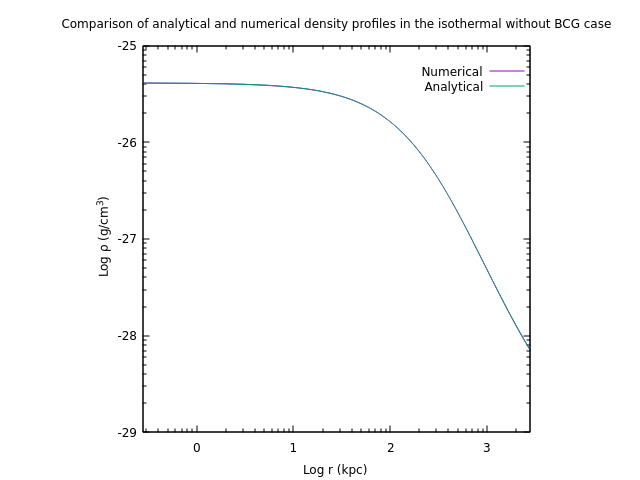
\includegraphics[width=\textwidth]{rhoiso.png}
	\caption{Comparison between the density profile obtained numerically for the isothermal model without the BCG (purple curve) and the analytical one given by \eqref{isogas} (green curve)}
	\label{fig:analvsnum}
\end{figure}
\begin{figure}[H]
	\begin{subfigure}{0.49\textwidth}
		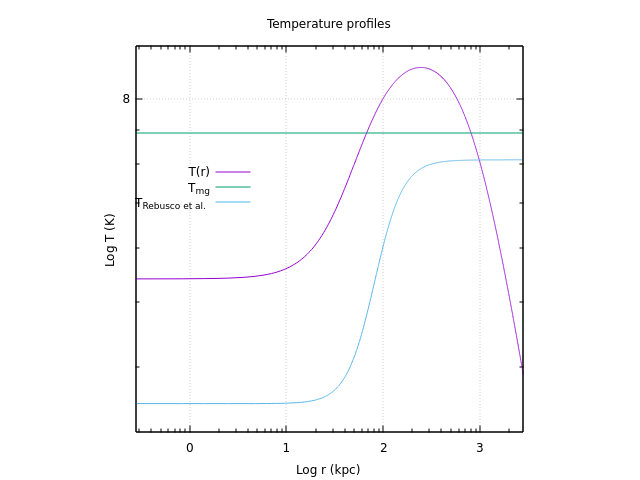
\includegraphics[width=\textwidth]{temprofiles.png}
	\end{subfigure}
	\begin{subfigure}{0.49\textwidth}
		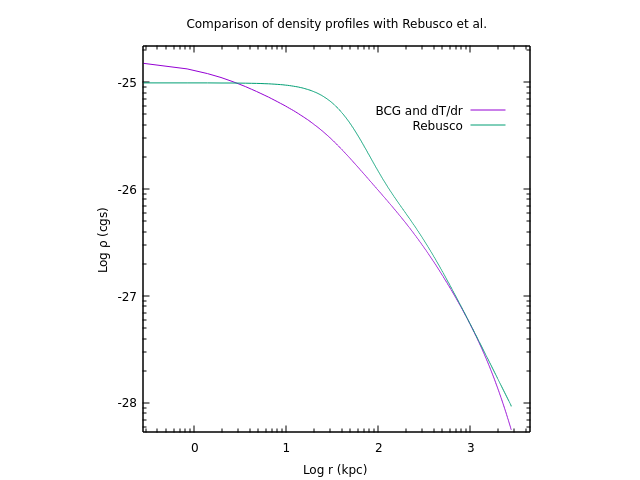
\includegraphics[width=\textwidth]{rebrho.png}
	\end{subfigure}
	\caption{On the left: the two gas temperature profiles adopted in the simulation. The purple curve represents the one given by \eqref{Tprof}, while the green line is the isothermal one. The light blue curve is a variable profile contained in \cite{rebusco}.
	On the right: the comparison between the density profile for the non isothermal model (purple curve) and the one contained in the aformentioned article }
	\label{fig:tempprof}
\end{figure}
FIg.\ref{fig:tempprof} shows both the adopted temperature profiles and the density profile obtained in the non-isothermal model compared to the temperature and density profile used in \cite{rebusco}, which are based on the deprojected $XMM-Newton$ data and are described by:
\begin{equation}
	T(r)=7\frac{1+(r/71)^{3}}{2.3+(r/71)^{3}}\text{keV},
\end{equation}
\begin{equation}
	\rho (r)=1.937\times 10^{-24}\left\{\frac{4.6\times 10^{-2}}{[1+(r/57)^{2}]^{1.8}}+\frac{4.8\times 10^{-3}}{[1+(r/200)^{2}]^{0.87}}\right\}\text{g/cm}^{3}.
\end{equation}
In both formulas the $r $ is in kpc. With that being said, the differences between in the mass profiles for the two cases where we consider the presence of the BCG come from the fact that the variable temperature profile is below the constant one below $\sim 60$ and beyond
$\sim 800$ kpc, which means that the gas is colder than the isothermal model and has thus a higher density and mass.

\section{The diffusion of Fe in the ICM}
\subsection{Physical model}


\subsection{The simulation}

\subsection{Results and discussion}


\section*{Conclusions}



\begin{thebibliography}{1}
	\bibitem{rebusco}
	P. Rebusco et al. “Impact of stochastic gas motions on galaxy cluster abundance profiles”.
In: Mon. Not. R. Astron. Soc. 359 (2005), pp. 1041–1048. doi: https://doi.org/10.
1111/j.1365-2966.2005.08965.x.
\end{thebibliography}
\end{document}